\documentclass{beamer}

% automatic section title page
\AtBeginSection[]{
  \begin{frame}
  \vfill
  \centering
  \begin{beamercolorbox}[sep=8pt,center,shadow=true,rounded=true]{title}
    \usebeamerfont{title}\insertsectionhead\par%
  \end{beamercolorbox}
  \vfill
  \end{frame}
}

\usepackage{concmath} 
\usetheme{Boadilla}
\usepackage[utf8]{inputenc}
\usepackage{helvet}
\usepackage[english]{babel}
\usepackage{hyperref}

\usepackage{natbib} % for the bibliography
% \setcitestyle{numbers}

\usecolortheme{tum}
\useoutertheme{tum}

\setbeamerfont{author}{size=\footnotesize}
\setbeamerfont{date}{size=\scriptsize}
\setbeamerfont{date}{size=\scriptsize}

\useinnertheme{rectangles}

\usepackage{pgf}  
\usepackage{tikz}
\logo{\pgfputat{\pgfxy(-0.2, 8.5)}{\pgfbox[right,top]{
\begin{tikzpicture}[y=0.38pt, x=0.38pt,yscale=-1, inner sep=0pt, outer sep=0pt]
\begin{scope}[cm={{1.25,0.0,0.0,-1.25,(0.0,35.4325)}}]
    \path[fill=tum,nonzero rule] (4.8090,23.2950) -- (4.8090,-0.0020) --
      (9.8590,-0.0020) -- (9.8590,23.2600) -- (15.4730,23.2600) -- (15.4730,-0.0020)
      -- (31.5390,-0.0020) -- (31.5390,23.0140) -- (37.2580,23.0140) --
      (37.2580,0.0060) -- (42.5550,0.0060) -- (42.5550,23.0140) -- (48.3440,23.0140)
      -- (48.3440,0.0060) -- (53.6410,0.0060) -- (53.6410,28.3460) --
      (26.4530,28.3460) -- (26.4530,5.1580) -- (20.6290,5.1580) -- (20.6290,28.3110)
      -- (-0.0000,28.3110) -- (-0.0000,23.2950) -- (4.8090,23.2950) -- cycle;
\end{scope}
\end{tikzpicture}
}}}

\setbeamertemplate{title page}
{
	\vbox{}
	\vfill
	\begin{flushleft}
		\begin{beamercolorbox}[sep=8pt,left]{title}
			\usebeamerfont{title}\inserttitle\par%
			\ifx\insertsubtitle\@empty%
			\else%
				\vskip0.25em%
				{\usebeamerfont{subtitle}\usebeamercolor[fg]{subtitle}\insertsubtitle\par}%
			\fi%
    	\end{beamercolorbox}%
    	\vskip1em\par
		\begin{beamercolorbox}[sep=8pt,left]{author}
		\usebeamerfont{author}\insertauthor
		\end{beamercolorbox}
		\begin{beamercolorbox}[sep=8pt,left]{institute}
		\usebeamerfont{institute}\insertinstitute
		\end{beamercolorbox}
		\begin{beamercolorbox}[sep=8pt,left]{date}
		\usebeamerfont{date}\insertdate
		\end{beamercolorbox}\vskip0.5em
		{\usebeamercolor[fg]{titlegraphic}\inserttitlegraphic\par}
	\end{flushleft}
	\vfill
}

\setbeamertemplate{caption}[numbered]

\mode<presentation>

\title{Automatic Music Transcription}
\subtitle{Overview, Onsets and Frames, Unaligned Supervision}

\author{Matilde Tozzi}
\institute[]{Ferienakademie}
\date[September 2024]{September 2024}

\newcommand{\emp}[1]{\textcolor{tum}{\textbf{#1}}}
\graphicspath{{.}{./Pictures/}}

\hypersetup{
  colorlinks   = true, %Colours links instead of ugly boxes
  urlcolor     = tum-darker, %Colour for external hyperlinks
  linkcolor    = tum, %Colour of internal links
  citecolor   = black %Colour of citations
}

\begin{document}
\beamertemplatenavigationsymbolsempty

% 1. Slide: Title
\begin{frame}
	\titlepage
\end{frame}

% 2. Slide: TOC
\begin{frame}
	\frametitle{Table of contents}
	\tableofcontents
\end{frame}


%%%%%%%%%%%%%%%%%%% Overview
\section{Overview}
\subsection{Definition}
\begin{frame}
	\frametitle{Definition}
	\begin{block}{}
		\emp{Automatic Music Transcription (AMT)} is the design of computational algorithms to convert acoustic music signals into some form of music notation. \cite{Overview}
	\end{block}

	\emp{Subtasks}:
	\begin{itemize}
		\item multipitch estimation
		\item onset and offset detection
		\item instrument recognition
		\item beat and rhythm tracking
		\item dynamics
		\item score typesetting
	\end{itemize}
\end{frame}

\subsection{Usual Workflow}
\begin{frame}[shrink=10]
	\frametitle{Usual Workflow}

	\begin{columns}

		\begin{column}{0.5\textwidth}
			\begin{itemize}
				\vspace{2mm}
				\item \emp{(a)} audio waveform as input
				      \vspace{2mm}
				\item \emp{(b)} time-frequency representation
				      \vspace{2mm}
				\item \emp{(c)} piano-roll (MIDI: Musical Instrument Digital Interface) representation as output
				      \vspace{2mm}
				\item \emp{(d)} typeset music score
			\end{itemize}
		\end{column}

		\begin{column}{0.5\textwidth}
			\begin{figure}[!ht]
				\centering
				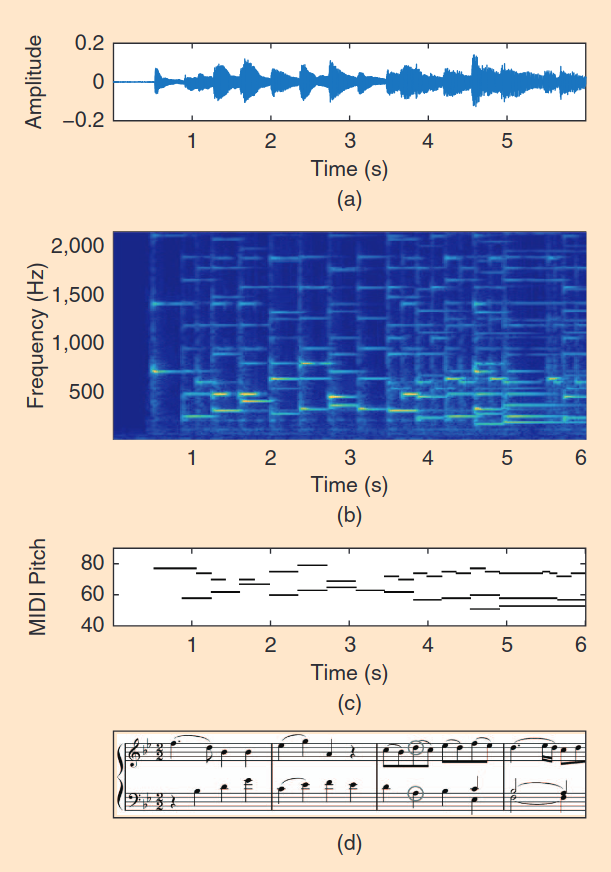
\includegraphics[width=.7\textwidth]{workflow.png}
				\caption{Source: \cite{Overview} (Images courtesy of the MIDI Aligned Piano Sound database).}
				\label{fig:workflow}
			\end{figure}
		\end{column}

	\end{columns}
\end{frame}


% \subsection{Applications}
% \begin{frame}
% 	\frametitle{Applications\footnote{\cite{Overview}}}
% 	\begin{itemize}
% 		\item music education (tutoring)
% 		\item music creation (dictation)
% 		\item music prodution (content visualization and editing)
% 		\item music search (indexing, recommendation by features)
% 		\item musicology (analysis of nonnotated music)
% 		\item music information retrieval (structural segmentations, cover-song detection, music similarity)
% 	\end{itemize}
% \end{frame}


\subsection{AMT Approaches}
\begin{frame}[shrink=10]
	\frametitle{AMT Approaches}

	\begin{columns}
		\begin{column}{0.5\textwidth}
			\begin{itemize}
				\item \emp{(a)} \textbf{frame level} = estimation of the number of and pitch of notes that are simultaneously present in each time frame ($\sim 10ms$), independently in each \textit{time frame}
				      \vspace{2mm}
				\item \emp{(b)} \textbf{note level} = connects pitch estimates over time into \textit{notes} (pitch, onset time, offset time)
				      \vspace{2mm}
				\item \emp{(c)} \textbf{stream level} (multipitch streaming) = grouping of estimated pitches or notes into \textit{streams} (one instrument or musical voice)
			\end{itemize}
		\end{column}

		\begin{column}{0.5\textwidth}
			\begin{figure}[!ht]
				\centering
				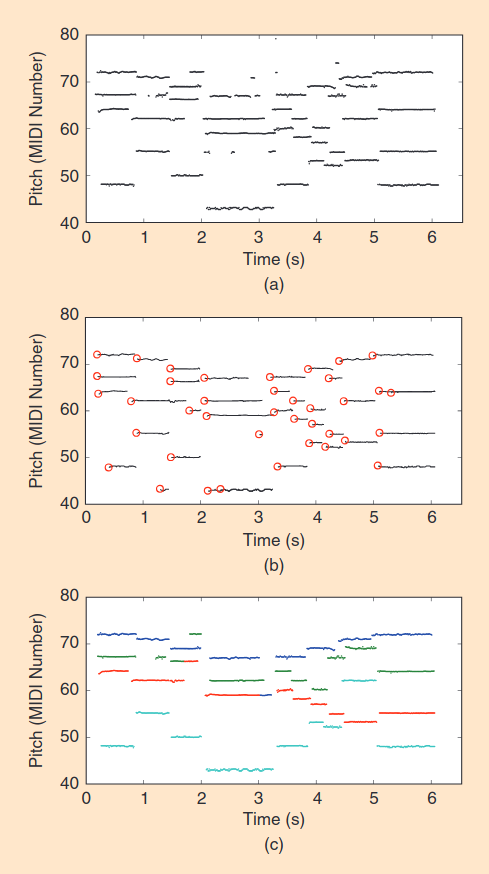
\includegraphics[width=.6\textwidth]{transcriptions.png}
				\caption{First phrase of J.S. Bach's chorale \textit{Ach Gott und Herr}. Source: \cite{Overview}.}
				\label{fig:transcriptions}
			\end{figure}
		\end{column}
	\end{columns}

\end{frame}

\subsection{State of the Art}
\begin{frame}[allowframebreaks]
	\frametitle{State of the Art}
	% \begin{enumerate}
	% \item \emp{Negative Matrix Factorization} (not covered in this seminar)

	%       Represent a given nonnegative time-frequency representation $\boldsymbol{V}\in\mathbb{R}_{\geq0}^{MxN}$ as a product of two nonnegative matrices: a \textbf{dictionary} $\boldsymbol{D}\in\mathbb{R}_{\geq0}^{MxK}$ and an \textbf{activation matrix} $\boldsymbol{A}\in\mathbb{R}_{\geq0}^{KxN}$. The goal is to minimize a distance (or divergence) between $\boldsymbol{V}$ and $\boldsymbol{DA}$ w.r.t. $\boldsymbol{D}$ and $\boldsymbol{A}$.
	%       \framebreak
	%       \begin{figure}[!ht]
	% 	      \centering
	% 	      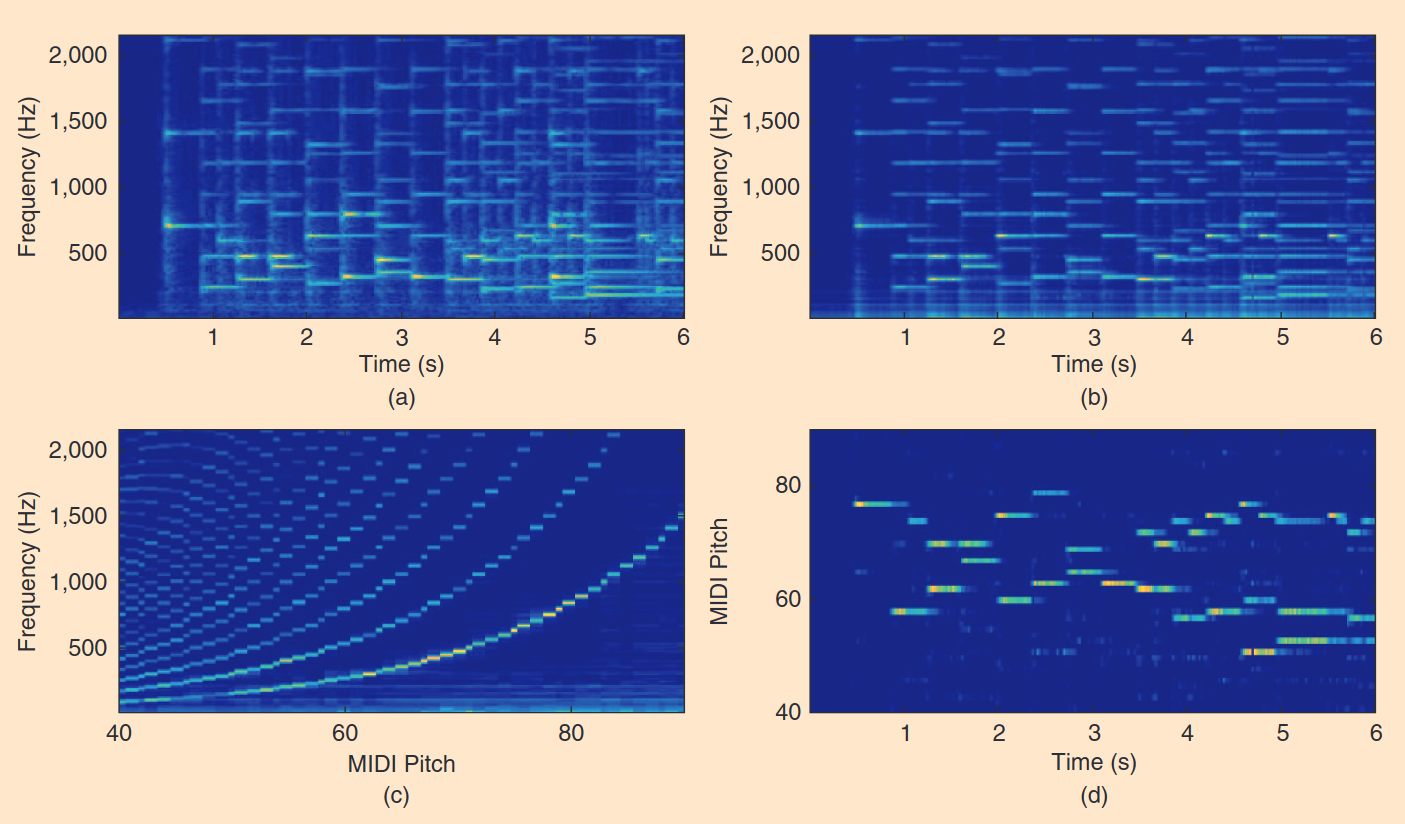
\includegraphics[width=.8\textwidth]{NMF.png}
	% 	      \caption{And example of NMF, using the same audio recording as in Figure \ref{fig:workflow}: \textbf{(a)} input spectrogram $\boldsymbol{V}$, \textbf{(b)} approximated spectrogram $\boldsymbol{DA}$, \textbf{(c)} dictionary $\boldsymbol{D}$, and \textbf{(d)} activation matrix $\boldsymbol{A}$. Source: \cite{Overview}.}
	% 	      \label{fig:NMF}
	%       \end{figure}
	%       \framebreak
	\emp{Neural Networks} %(focus of this seminar)



	\begin{columns}
		\begin{column}{0.4\textwidth}
			The most popular approach of this type is called \textbf{Onsets and Frames}, because it consists of two chained NNs. One detects \textit{note onset}, and its outuput is used to inform a second network that focuses on perceiving the \textit{note lengths}.
		\end{column}

		\begin{column}{0.6\textwidth}
			\begin{figure}[!ht]
				\centering
				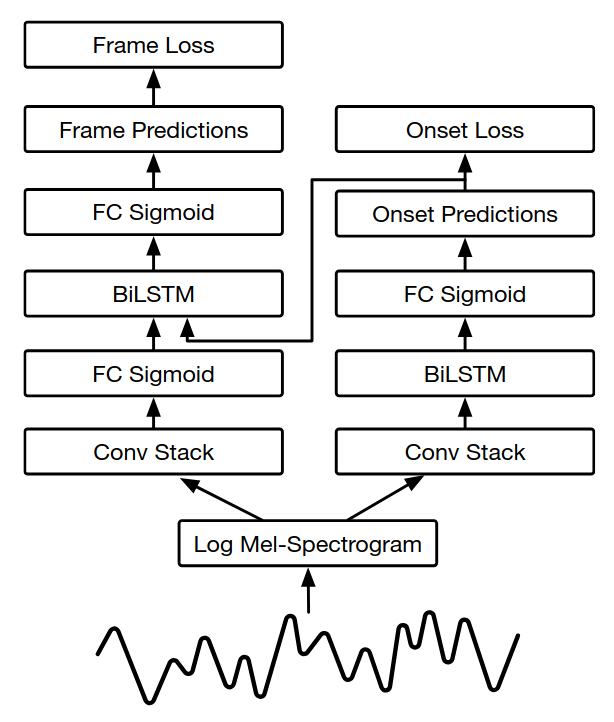
\includegraphics[width=.7\textwidth]{OF.png}
				\caption{Source: \cite{OF}.}
				\label{fig:OF}
			\end{figure}
		\end{column}
	\end{columns}



	% \end{enumerate}

	\framebreak

	\begin{block}{Mel-Spectrogram}
		The \emp{mel scale} (after the word \textit{melody})
		is a perceptual scale of pitches judged by listeners to be equal in distance from one another.

		\begin{itemize}
			\item Reference point: 1000 mels = 1000 Hz tone, 40 dB above the listener's threshold.
			\item Above about 500 Hz, increasingly large intervals are judged by listeners to produce equal pitch increments.
		\end{itemize}



	\end{block}

	\framebreak

	\begin{equation*}
		m = 2595\log_{10}\left(1+\frac{f}{700}\right)
	\end{equation*}

	\begin{figure}[!ht]
		\centering
		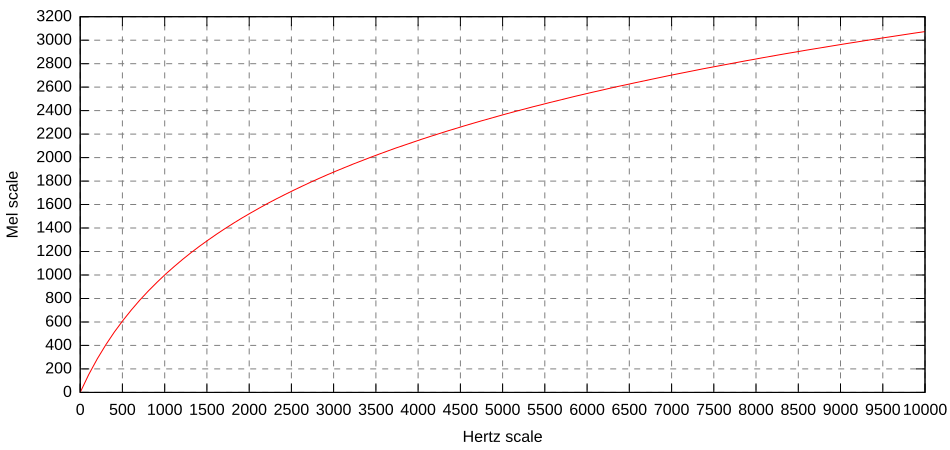
\includegraphics[width=.9\textwidth]{Mel-Hz_plot.png}
		\caption{Relation between Hertz and Mel scales. Source: \cite{MEL}.}
		\label{fig:mel}
	\end{figure}


	% \framebreak

	% \begin{figure}[!ht]
	% 	\centering
	% 	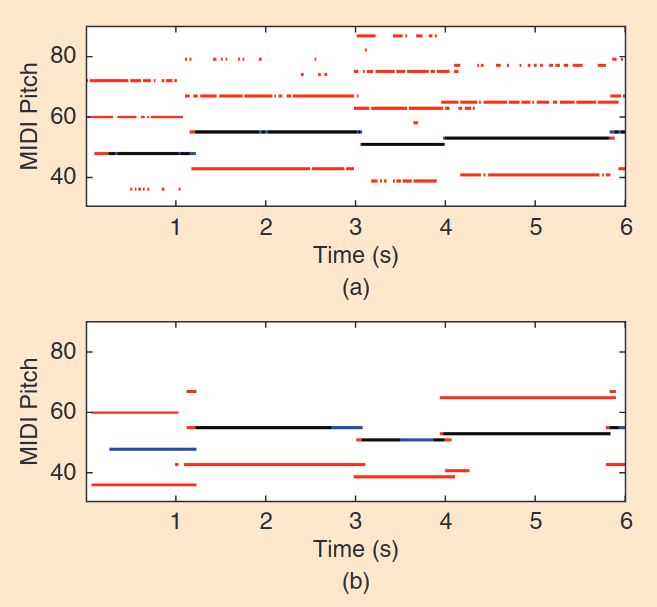
\includegraphics[width=.5\textwidth]{comparison.png}
	% 	\caption{Piano-roll representation of the first 6s of a recording of a Bach piece (BWV 582) for the organ. \textbf{(a)} is a NMF model, \textbf{(b)} is a NN model, both trained on the piano. Source: \cite{Overview}.}
	% 	\label{fig:comparison}
	% \end{figure}

\end{frame}

\subsection{Key Challenges}
\begin{frame}
	\frametitle{Key Challenges\footnote{\cite{Overview}}}
	\begin{enumerate}
		\item multiple simultaneous sources
		\item harmonic relations in overlapping sounds
		      \begin{itemize}
			      \item C major chord, fundamental frequency ratio C:E:G 4:5:6
			      \item harmonic overlap 46.7\%, 33.3\%, 60\% for C, E, and G respectively
		      \end{itemize}
		\item high synchronization of onsets and offsets between different voices $\Rightarrow$ no statistical independence between sources
		\item annotation is very time consuming and requires high expertise
		      \begin{itemize}
			      \item sheet music is not a good ground-truth: not time-aligned, not an accurate performance representation
		      \end{itemize}
	\end{enumerate}

	\emp{Examples of metric limitations for Osets and Frames\footnote{\cite{OF}}}

	\href{https://storage.googleapis.com/magentadata/papers/onsets-frames/fur_elise_framescore_good2.mp3}{Original Score}

	\href{https://storage.googleapis.com/magentadata/papers/onsets-frames/fur_elise_notejitter_score1.mp3}{Note timing jittered, but still within tolerance}

	\href{https://storage.googleapis.com/magentadata/papers/onsets-frames/fur_elise_framescore_bad3.mp3}{Many 1-frame notes added}

\end{frame}

%%%%%%%%%%%%%%%%%%% AMT

\section{Unaligned Supervision for AMT in the Wild}

\subsection{Scheme}
\begin{frame}
	\frametitle{Scheme}

	\begin{figure}[!ht]
		\centering
		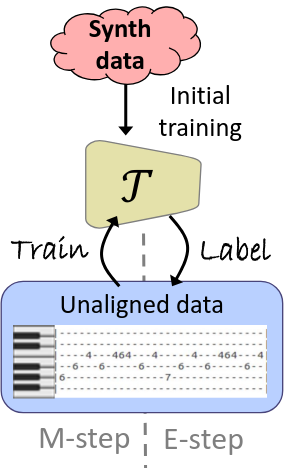
\includegraphics[width=.2\textwidth]{AMT-general.png}
	\end{figure}

	\begin{figure}[!ht]
		\centering
		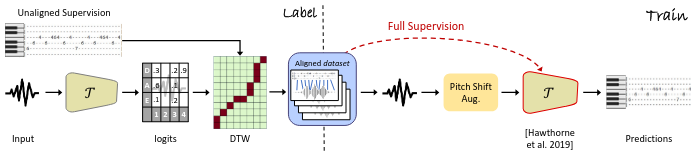
\includegraphics[width=.9\textwidth]{AMT-scheme.png}
		\caption{Source: \cite{AMT}.}
		\label{fig:AMT-scheme}
	\end{figure}

\end{frame}































%%%%%%%%%%%%%%%%%%% Bibliography
\begin{frame}[shrink=5]
	\frametitle{Bibliography}

	% A special thanks to \emp{Abhirup Saha} for the slides on the topic.

	% \vspace{5mm}

	\bibliographystyle{alpha}
	\begin{thebibliography}{BenetosMusicTranscription}

		\bibitem[BenetosMusicTranscription]{Overview}
		E. Benetos, S. Dixon, Z. Duan, and S. Ewert, “Automatic Music Transcription: An Overview,” IEEE Signal Processing Magazine, vol. 36, no. 1, pp. 20–30, Jan. 2019, doi: \url{https://doi.org/10.1109/msp.2018.2869928}.

		\bibitem[HawthorneOnsetsFrames]{OF}
		C. Hawthorne et al., “Onsets and Frames: Dual-Objective Piano Transcription,” International Symposium/Conference on Music Information Retrieval, pp. 50–57, Sep. 2018, doi: \url{https://doi.org/10.5281/zenodo.1492341}.

		\bibitem[MamanUnalignedAMT]{AMT}
		B. Maman and A. Bermano, “Unaligned Supervision for Automatic Music Transcription in-the-Wild.”

		\bibitem[MelScale]{MEL}
		\url{https://en.wikipedia.org/wiki/Mel_scale}

	\end{thebibliography}
\end{frame}

\end{document}